\section{Apresentação}

\begin{frame}	
	\begin{block}{Apresentação}	
		\begin{itemize}
			\item Adilson Khouri,  jogador de Magic the Gathering, nerd, apaixonado por computação e machine learning!
		\end{itemize}
		 \begin{figure}[!htb]
			\centering	  				
			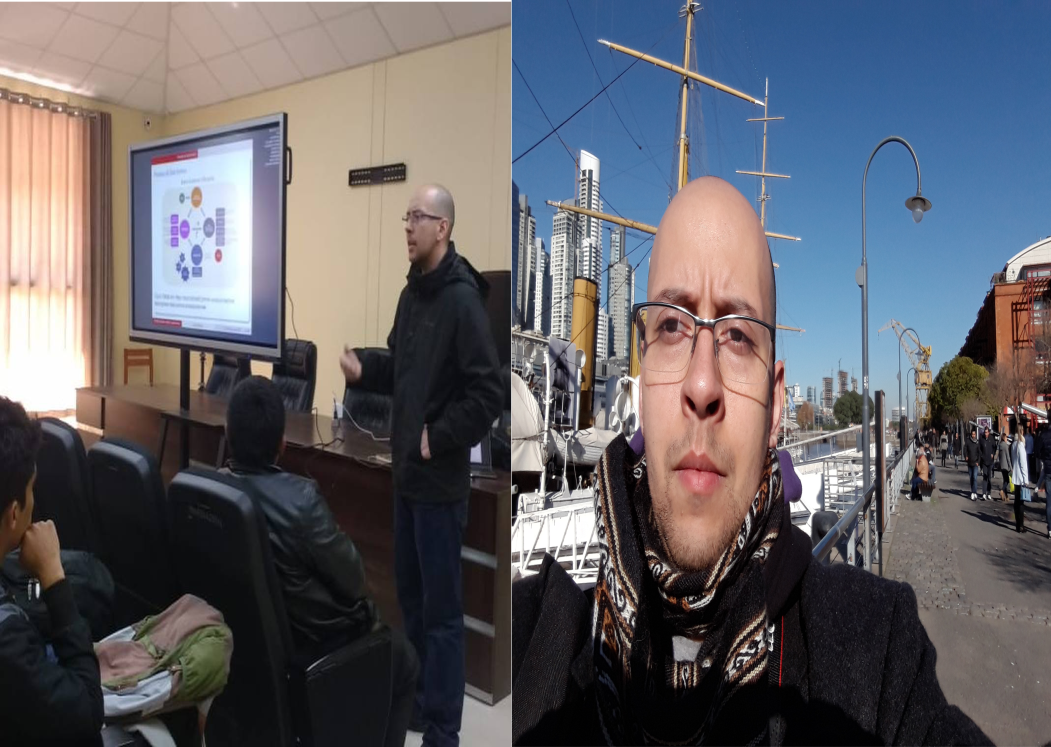
\includegraphics[height=4cm, width = 7cm]{./pic/image3460.png}
			\caption{Ministrando uma palestra no Peru e trabalhando na Argentina}
			\label{fig_adilson_argentina}
		\end{figure}
	\end{block}
\end{frame}
			
\begin{frame}	
	\begin{block}{Formação Acadêmica}
		 \begin{itemize}
			  \item Bacharel em Sistemas de Informação (2011 - USP)
			  \item Mestre em Sistemas de Informação (2016 - USP)
			  \item Doutorando em Sistemas de Informação (cursando - USP)
		  \end{itemize}
	\end{block}
\end{frame}

\begin{frame}	
	\begin{block}{Experiência Acadêmica}
		 \begin{itemize}
			  \item Um ano de estágio em docência na USP
			  \item Publicações Científicas
			  \item Orientação de iniciação científica
			  \item Disciplina: "Técnicas de programação em Games" (SENAC)
			  \item Disciplina: "TCC 2"	(SENAC)
		  \end{itemize}
	\end{block}
\end{frame}

\begin{frame}	
	\begin{block}{Experiência de Mercado}
		\begin{itemize}
			\item Programador na consultoria Arbit (2010-2011)
			\item Programador Itaú-Unibanco (2011-2013)
			\item Cientista de dados Sr. PagSeguro (2016 - 2018)
			\item Cientista de dados Sr. NuvemShop (Atual)
			\item Professor de Programação - SENAC (Atual)
		\end{itemize}
	\end{block}
\end{frame}

\begin{frame}	
	\begin{block}{E os senhores?}
		\begin{itemize}
			\item Nome
			\item Graduação / pós-graduação
			\item Trabalho
			\item Qual sua experiência com os tópicos dessa disciplina?
		\end{itemize}
	\end{block}
\end{frame}

\begin{frame}	
	\begin{block}{Expectativas}
		\begin{itemize}
			\item Quais expectativas?
			\item O que deve ser evitado?
			\item (E-Mail: 0800dirso@gmail.com)
		\end{itemize}
	\end{block}
\end{frame}